%
% A2
%
\chapter{Mathematical notation}%
  %
  %
  \label{ch:math}%
	\index{Mathematical notation}%
	%
	%




Many aspects of human survival are related to events, objects or people that can be enumerated. For example, infant mortality, forced migration and market collapse are all quantifiable social problems for which we might want to know how frequently they occur, and under what circumstances. A lot of applied mathematics is therefore used in the formalization of markets, populations and disease, both for industrial and for research purposes.

To manipulate things in mathematical form, we rely on symbols and conventions to write down expressions like $y = f(x)$ (the function $f$ that returns the value $y$ for a value of $x$).

\paragraph{Greek letters}%
%
Table~\ref{tbl:greek} references the Greek letters that are used in conventional notation: if you read a lot of science-fiction, you might be able to skip this, otherwise start familiarizing yourself with them. In practice, we will use only a subset of the Greek alphabet, and we will use only a few letters at a time.

\begin{table}%

$$
\begin{array}{r*5lrl}
\multicolumn{6}{l}{\text{\textbf{Lowercase}:}} &\multicolumn{2}{l}{\text{\textbf{Uppercase}:}}\\[.5em]
\alpha		& \text{alpha}			& \kappa	& \text{kappa}			& \tau		& \text{tau}		& \Gamma		& \text{Gamma} \\
\beta		& \text{beta}			& \lambda	& \text{lambda}			& \upsilon	& \text{upsilon}	& \Delta		& \text{Delta} \\
\gamma		& \text{gamma}			& \mu		& \text{mu}				& \phi		& \text{phi}		& \Theta		& \text{Theta} \\
\delta		& \text{delta}			& \nu		& \text{nu}				& \varphi	& \text{var-phi}	& \Lambda		& \text{Lambda} \\
\epsilon	& \text{epsilon}  		& \xi		& \text{xi}				& \chi		& \text{chi}		& \Xi			& \text{Xi} \\
\varepsilon	& \text{var-epsilon}	& \pi		& \text{pi}				& \psi		& \text{psi} 		& \Pi			& \text{Pi} \\
\zeta		& \text{zeta}			& \varpi	& \text{var-pi}			& \omega	& \text{omega}		& \Sigma		& \text{Sigma} \\
\eta		& \text{eta}			& \rho		& \text{rho}			&			&					& \Upsilon		& \text{Upsilon} \\
\theta		& \text{theta}			& \varrho	& \text{var-rho}		&			&					& \Phi			& \text{Phi} \\
\vartheta	& \text{var-theta}		& \sigma	& \text{sigma}			&			&					& \Psi			& \text{Psi} \\
\iota		& \text{iota} 			& \varsigma	& \text{var-sigma}		&			&					& \Omega		& \text{Omega}
\end{array}
$$
  
  \caption{Greek letters}\label{tbl:greek}
\end{table}

% You can read sequences of letters and numbers by simple enunciation: $\Delta x$ is pronounced ``delta-x'' and $\beta_1X_1$ is pronounced ``Beta-One X-One''. Note that the pronunciation of Greek letters varies from your linguistic standard: $\chi^2$, for example, designates the ``Chi-squared'' value, which is pronounced ``Kai-squared''.

\paragraph{Mathematical symbols}%
%
Table~\ref{tbl:math} references some common math symbols that are used to compose expressions such as: for every ($\forall$) nonnegative real number $(x \in \mathbb{R}^{+})$, there exists ($\exists$) a square root number given by the function $f: x \rightarrow \sqrt{x}$. Again, we will use only a few of these symbols for demonstration purposes.

\begin{table}%

$$
\begin{array}{rlrlrlrl}
\exists  	    & \text{there exists}	            & |x|      	  & \text{absolute value, determinant}			& \Sigma      & \text{summation}              \\
\forall		    & \text{for all/any}	            & [...]       & \text{closed interval}			            & \Pi         &  \text{product}               \\
\therefore		& \text{therefore}	              & (...)       & \text{open interval}    				        & \Delta x    & \text{the change in } x       \\
\Rightarrow		& \text{implies}			            & \{...\}     & \text{set}	                  			    & \partial	  & \text{partial differential}   \\
\to  & \text{goes to, approaches}  	            & \varnothing & \text{empty set}      		              & \int		    & \text{integral}               \\
\mid          & \text{such that, given}     	  & \subseteq   & \text{is a subset of}       			      & x!		      & \text{factorial}              \\
\text{iff}    & \text{if and only if}			      & \subset     & \text{is a proper subset of}			      & \ln(x)	    & \text{natural logarithm}      \\
\in           & \text{is an element of}		      & \cup        &	\text{union}                            & \log_b(x)		& \text{logarithm of base } b   \\
\notin        & \text{is not an element of} 		& \cap		    &	\text{intersection}                     &	x^k   	    & x \text{ at power/exponent } k\\
\approx       & \text{equals approximately}     & \infty      & \text{infinity}                         & \sqrt{x}    & \text{square root of } x      \\
\simeq        & \text{approximately equal to}   & \lim        & \text{limit}                            & \sqrt[3]{x} & \text{cubic root of } x       \\
\end{array}
$$
  
  \caption{Selected mathematical symbols and expressions}\label{tbl:math}
\end{table}


Some letters have standard representations in statistics, such as $\mu$ and $\bar X$ for the population and sample means, $\sigma$ and $s$ for standard deviation, $\sigma^2$ and $s^2$ for variance, etc. You will learn these conventions through practice. Using a computer will introduce slight deviations to these conventions because statistical software like Stata might denote, for instance, $\chi^2$ as \texttt{chi(2)}.

\paragraph{Numbers}%
%
Positive numbers like $7, 4, 5$ (the $+$ sign can be omitted) and negative numbers like $-10, -3$ are called integers. These numbers can be ordered to form a coordinate system centred around $0$, as shown below:

% \begin{figure}[h]
%   \begin{tikzpicture}[x=0.75cm,>=stealth]
%     \draw[<->] (-5,0)--(5,0);
%     \foreach \x in {-4,...,4}
%     \draw[shift={(\x,0)},color=black] (0pt,2pt) -- (0pt,-2pt) node[below] {\footnotesize $\x$};
%     \node[below] at (-5,-5pt) {$\ldots$};
%     \node[below] at (5,-5pt) {$\ldots$};
%   \end{tikzpicture}
% \end{figure}

The numbers covered by that coordinate system are said to be rational if they can be expressed as a ratio of two integers $r = \frac{n}{d}$ with $d \neq 0$. Numbers that cannot take the form of a ratio, like $\sqrt{2}$ or the mathematical constant $e$, are said to be irrational.

Rational and irrational numbers form the set $\mathbb{R}$ of real numbers, which is the set that we will use to explore calculus. This set designates a system of coordinates that is called the real number line, which we will use for variable construction and visualization:

\begin{figure}[h]
  \begin{tikzpicture}[x=0.75cm,>=stealth]
    \draw[<->] (-5,0)--(5,0);
    \foreach \x in {-4,...,4}
    \draw[shift={(\x,0)},color=black] (0pt,2pt) -- (0pt,-2pt) node[below] {\footnotesize $\x$};
    \node[above,color=s1] at (7.5,15pt)  {irrational numbers};
    \draw[color=s1] (1.41,0) -- (1.41,15pt);
    \node[above,color=s1] at (1.41,15pt) {$\sqrt{2}$};
    \draw[color=s1] (2.71,0) -- (2.71,15pt);
    \node[above,color=s1] at (2.71,15pt) {$e$};
    \node[below,color=s2] at (7.5,-15pt)  {rational numbers};
    \draw[color=s2] (-1/2,0) -- (-1/2,-15pt);
    \node[below,color=s2] at (-1/2,-15pt) {$-\frac{1}{2}$};
    \draw[color=s2] (9/4,0) -- (9/4,-15pt);
    \node[below,color=s2] at (9/4,-15pt) {$\frac{9}{4}$};
    \node[below] at (-5,-5pt)  {$\ldots$};
    \node[below] at (5,-5pt)   {$\ldots$};
  \end{tikzpicture}
  \caption{The real number line.}
\end{figure}

Intervals. Cartesian planes.

\section*{Exponents and logarithms}

\subsection{Power functions}

Power functions feature an exponent $k$ to raise $x$ to a given power, such that $f(x) = x^k = x*x*...*x$ ($k$ times). Some examples of power functions, where the exponent is constant, are shown in Figure~\ref{fig:exps-and-powers}.

\paragraph{Example: Scientific notation}%
%
Power functions are useful to rewrite large numbers with the function $f: x \to a \times 10^b$, where $a$ is any real number and $b$ is an integer. For example, by the end of August 2012, the U.S. national debt amounted to \$\href{http://www.treasurydirect.gov/NP/BPDLogin?application=np}{16,015,769,788,215.80}. This number can also be written as $16 \times 10^{12}$, i.e. 16 trillion, or as \ensuremath{1.6\times 10^{13}} in scientific notation.

Exponential functions are also useful to handle some phenomena like the exponential growth of the population or labour force in many countries, or the exponential decay of an organism or technology.

\begin{knitrout}
\definecolor{shadecolor}{rgb}{0.969, 0.969, 0.969}\color{fgcolor}\begin{figure}[]

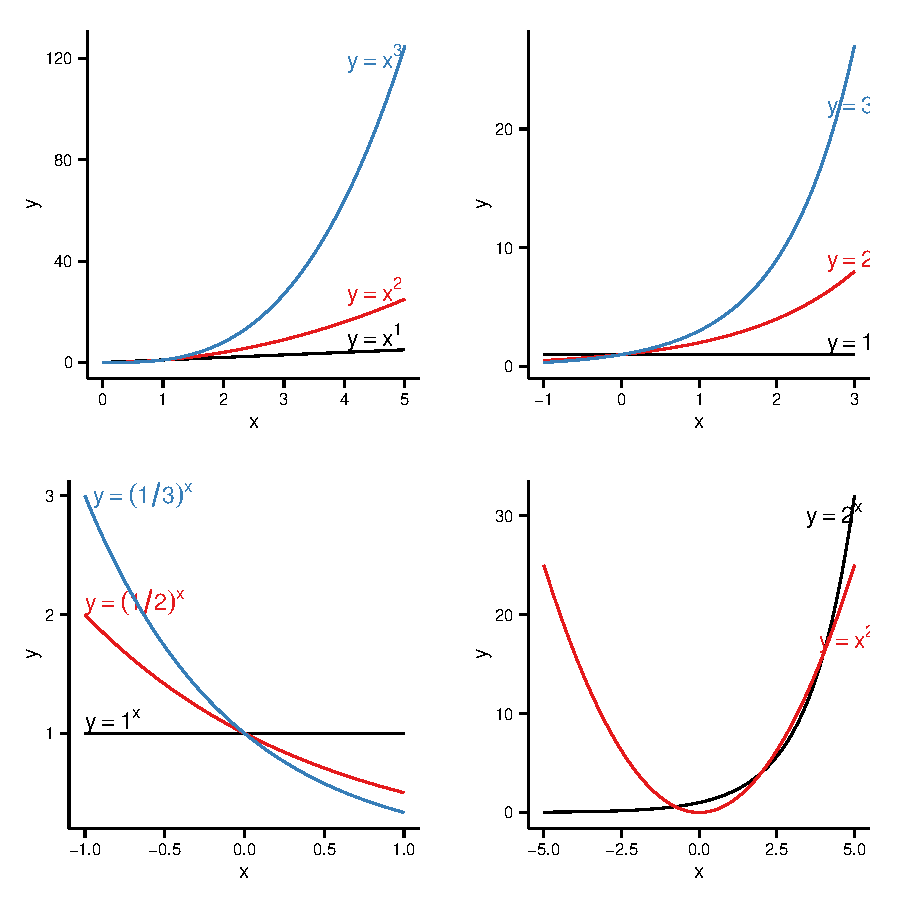
\includegraphics[width=\linewidth]{images/math-exps-and-powers} \caption{Top-left: visualization of the power functions $y = x^k$ for $k = [1,2,3]$. In the case where $k = 1$, the growth of $y$ is linear because $y = x$. All three curves are examples of strict monotonicity, i.e. a systematic increase of $y$ when $x$ increases. Top-right: exponential functions. Bottom-left: positive fractional exponentials (decay functions). Bottom-right: comparison of power and exponential progression near $0$.\label{fig:exps-and-powers}}
\end{figure}


\end{knitrout}


\subsection{Logarithms}

Logarithms are a way to reverse the transformation of an exponential function: $y = log_b x \iff b^y = x$. The logarithm can take any base $b > 0$.

\paragraph{Example: $y = \log_2(x)$} %
%
Early game consoles were often advertised through their bit ratings, which progressed exponentially from 8-bit to 64-bit processors. The geometric progression of their corresponding exponential function, $y = 2^x$, can also be described as the linear progression of its logarithm of base 2:

\begin{itemize}
  \item $y(3) = 2^3 = 8$ \quad then, by definition: \quad $\log_2(8) = 3$
  \item $y(4) = 2^4 = 16$ \quad then, by definition: \quad $\log_2(16) = 4$
  \item $y(5) = 2^5 = 32$ \quad then, by definition: \quad $\log_2(32) = 5$
  \item $y(6) = 2^6 = 64$ \quad then, by definition: \quad $\log_2(64) = 6$
\end{itemize}

The natural logarithm of base $e$ is denoted $\ln(x)$ or simply $\log(x)$, such that $\ln(x)=e^x$.

\begin{knitrout}
\definecolor{shadecolor}{rgb}{0.969, 0.969, 0.969}\color{fgcolor}\begin{figure}[]

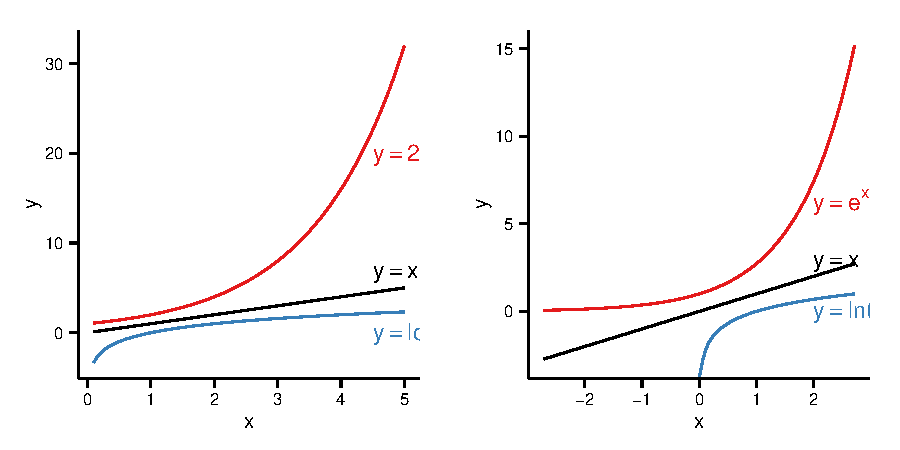
\includegraphics[width=\linewidth]{images/math-exps-and-logs} \caption{Left: logarithmic vs. exponential functions. Right: natural logarithm vs. exponential functions.\label{fig:exps-and-logs}}
\end{figure}


\end{knitrout}


Hi.

% Another application is the (heavily subsidised) production of ethanol in the United States, which has grown quasi-exponentially during the 20th century.
% http://www.graphoftheweek.org/2012/02/massive-increase-in-ethanol-production.html
% http://www.graphoftheweek.org/2012/06/body-weight-in-united-states-part-3.html
